% CHAPTER 5: Layer normalisation
\chapter{Layer Normalization}

\begin{figure}[H]
    \centering
    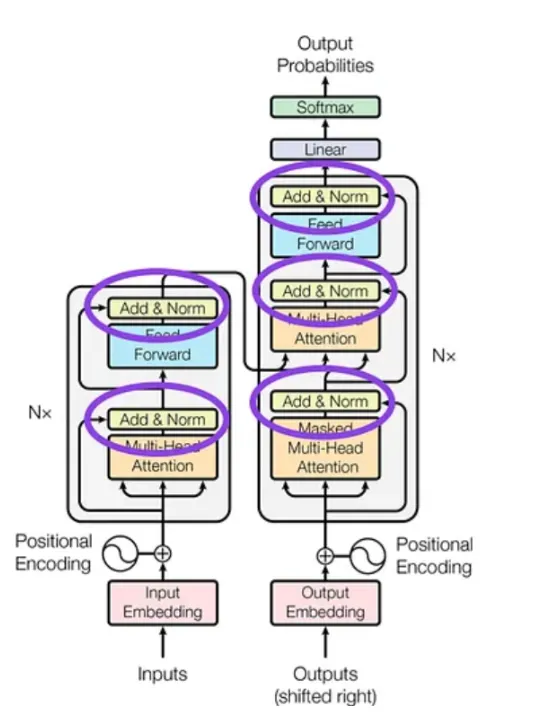
\includegraphics[width=0.4\linewidth]{Layer-normalization/architecture-layer-normalisation.png}
    \caption{Layer normalization in transformer architecture}
\end{figure}

Normalization in deep learning refers to the process of transforming data to have specific statistical properties. In deep learning, normalization can be applied in two key areas:
\begin{enumerate}
    \item \textbf{Input Data:} The data that you feed into the neural network, for example, features like \(f_1, f_2, f_3\), can be normalized before entering the network. This step is similar to what you have done in traditional machine learning.
    \item \textbf{Hidden Layer Activations:} You can also normalize the activations, i.e., outputs from hidden layers in the neural network. This is often done to stabilize and accelerate training, especially in deep networks.
\end{enumerate}

Let's dive into why normalization is required.

% Why normalisation
\section{Why is normalization required?}

Imagine that we are training a neural network, and as the weights are updated, some of them start getting really big. When that happens, the activations tied to those weights also become large, making it harder for the model to learn effectively. It slows things down and can cause problems in training.

Normalization helps fix this by keeping activations within a stable range. This not only makes the training process more stable but also speeds it up, allowing the model to learn more efficiently.

Another big benefit of normalization is that it prevents a problem called \textit{internal covariate shift} (discussed in the next section). On top of that, some types of normalization, like batch normalization, even help with regularization, which means the model can generalize better to new data.

Now that we’ve got an idea of why normalization is important, let’s move on to a quick review of batch normalization.

% Batch normalisation
\section{Recap of batch normalization}

\subsection{What is internal covariate shift?}

Batch normalization is designed to address a specific problem known as \textbf{internal covariate shift}. To understand this, imagine a neural network with multiple hidden layers. During training, the distribution of activations in these layers can change because the weights are updated. This shifting distribution makes it challenging for the network to learn effectively, leading to unstable training.

Batch normalization mitigates this issue by normalizing the activations within each layer, ensuring they follow a consistent distribution with a mean of zero and a standard deviation of one.

\subsection{How does batch normalization work?}

Consider that we have a dataset with features $f_1$ and $f_2$ and a neural network with one hidden layer. We are processing the data in batches. The goal is to apply batch normalization to the output of the nodes in the hidden layer. For simplicity, let’s assume our batch size is 5. This means we will feed 5 rows of data to the neural network at once (NOTE: All the values below are randomly assigned).
\begin{figure}[H]
    \centering
    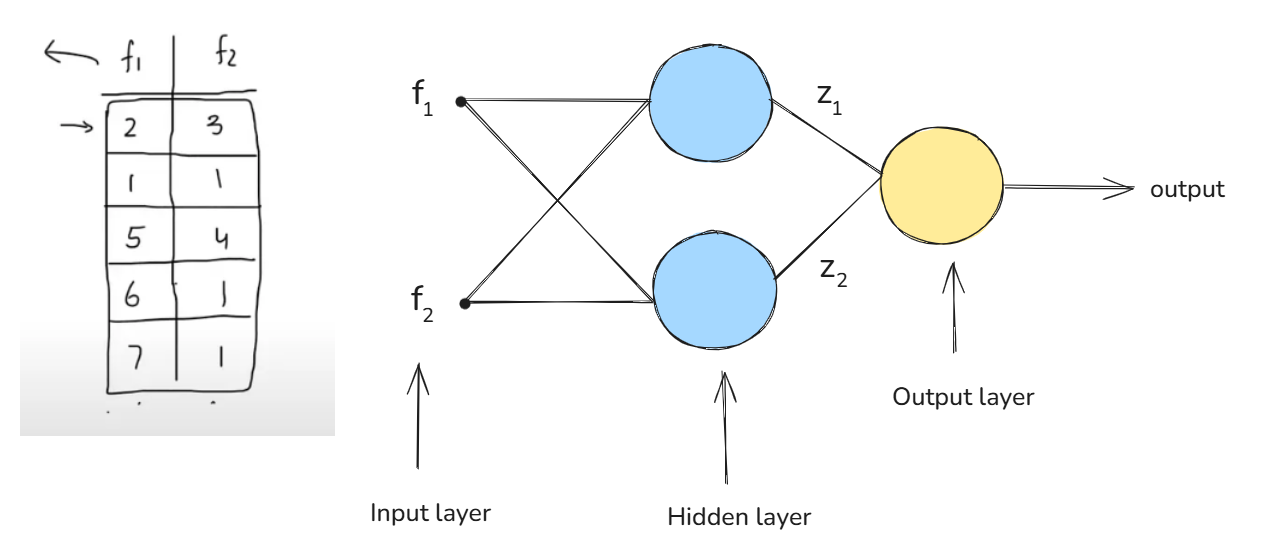
\includegraphics[width=0.5\linewidth]{Layer-normalization/batch-normalisation.png}
    \caption{Batch normalization setup}
\end{figure}

\textbf{Step 1: Calculating activations}\\
For each row in the batch, we calculate the activations for the nodes in the hidden layer. Since there are 2 nodes, we calculate activations $z_1$ and $z_2$.
\begin{figure}[H]
    \centering
    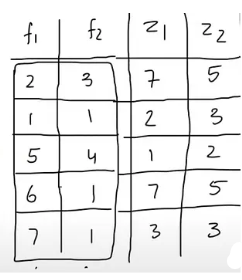
\includegraphics[width=0.3\linewidth]{Layer-normalization/activations.png}
    \caption{Calculating activations}
\end{figure}

\textbf{Step 2: Normalizing activations}
\begin{itemize}
    \item We compute the mean $(\mu)$ and standard deviation $(\sigma)$ for each activation value across the batch. For $z_1$, it is $(\mu_1, \sigma_1)$ and for $z_2$, it is $(\mu_2, \sigma_2)$.
    \item We normalize each activation using:
    $$\text{Normalized value} = \frac{\text{Original value} - \mu}{\sigma}$$
\end{itemize}

\textbf{Step 3: Scaling and shifting}\\
After normalization, we apply scaling and shifting. Each node has two learnable parameters: $\gamma$ and $\beta$.
$$\text{Final value} = (\text{Normalized value} \times \gamma) + \beta$$

Here, $\gamma$ and $\beta$ are initially set to 1 and 0, respectively, but are adjusted during training.

\textbf{Step 4: Applying activation function}\\
We replace the original activation values with the normalized values and pass the values through the activation function to get the final output for each node.

% Why batch normalisation is not used on sequential data
\section{Why can't we apply batch normalization to sequential data?}

Let us understand why we cannot apply batch normalization to sequential data. Up until now, we have considered feeding one sentence at a time into the self-attention module. But what if we want to process multiple sentences simultaneously? Let us say that we have decided to process two sentences at a time — meaning our batch size is set to two.

Let us consider these 2 sentences:\\
\textbf{Sentence 1:} Hi Nitish
\textbf{Sentence 2:} How are you today?\\

Each word in these sentences is represented by an embedding vector and for simplicity, let us keep the dimensionality of each embedding vector as 3.
\begin{figure}[H]
    \centering
    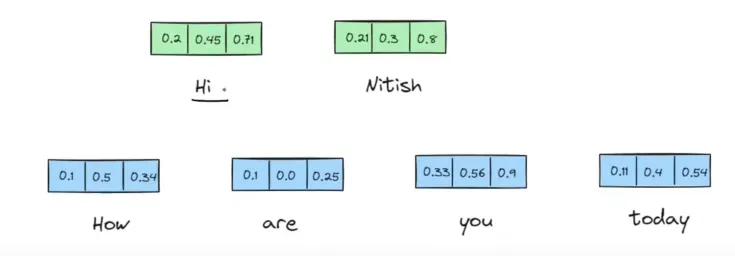
\includegraphics[width=0.6\linewidth]{Layer-normalization/batch-normalisation-sequential.png}
    \caption{Embedding vector of words}
\end{figure}

These sentences vary in length — one has 2 words, and the other has 4. However, in self-attention, we need to ensure that the number of words (tokens) in each sentence is equal when processing them together. This is where padding comes in.
\begin{figure}[H]
    \centering
    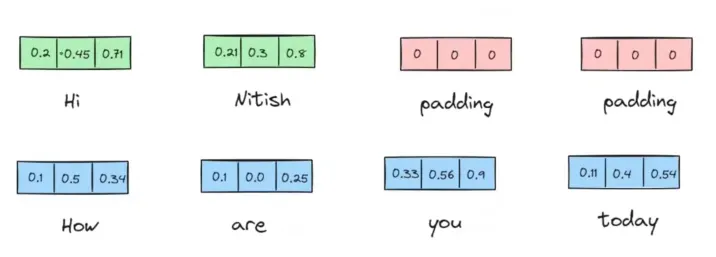
\includegraphics[width=0.5\linewidth]{Layer-normalization/padding-batch-normalisation.png}
    \caption{Padding}
\end{figure}

With both sentences now of equal length, they can be fed into the self-attention module. This module will calculate contextual embeddings for each word based on the entire sequence. The above embeddings can be represented using matrices. After passing the matrices through the self-attention block, we will obtain the contextual embeddings.
\begin{figure}[H]
    \centering
    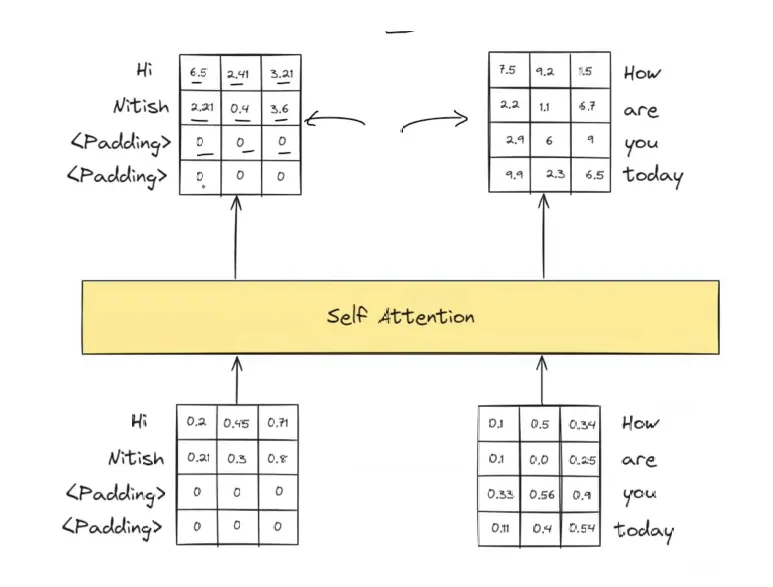
\includegraphics[width=0.5\linewidth]{Layer-normalization/contextual-embeddings-batch-normalisation.png}
    \caption{Contextual embeddings}
\end{figure}

Now, we stack both contextual embeddings together, as shown below:
\begin{figure}[H]
    \centering
    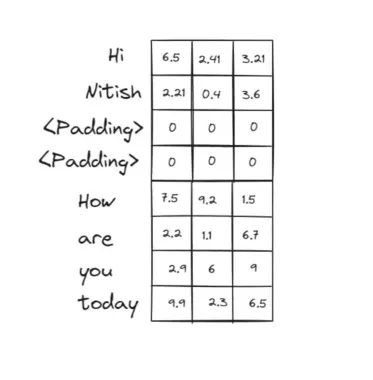
\includegraphics[width=0.5\linewidth]{Layer-normalization/stacking-batch-normalisation.png}
    \caption{Stacking the outputs}
\end{figure}

 Let’s apply batch normalization to this setup. An important point to note is that there are many zeros present in the data. If we have multiple zeros, the mean and variance that we calculate are not \textit{representative} of the actual data. It significantly affects how batch normalization works. This is the main issue.

% Layer normalisation
\section{The idea of layer normalization}

Consider that we have the same previous setup. We have the same neural network and data, so the foundation is consistent. We are still calculating $z_1$ and $z_2$, which represent the pre-activation values for the first and second node, respectively, for all data points.

One key similarity is that each node has its own $\gamma$ and $\beta$ parameters. The main difference arises in how normalization is applied. In batch normalization, the normalization is done across the batch (rows). But with layer normalization, normalization occurs across the features (columns).

To compute $\mu$ and $\sigma$, we calculate them for each row across all features. For instance, we compute $\mu_1$ and $\sigma_1$ for the first row, then $\mu_2$ and $\sigma_2$ for the second row. The rest of the process remains the same as in batch normalization.

This ensures that only the original data points are considered for calculating $\mu$ and $\sigma$. The mean and standard deviation across the features in rows with zero values are also 0. Hence, it is a better representation of the actual data. This enhances the model's performance and stability.

\textbf{NOTE:} The entire implementation can be found in this \underline{\href{https://colab.research.google.com/drive/1dJItP6qJuaUi4b-uDvZM9G_U6wCeXhbs?usp=sharing}{notebook}}